\documentclass{article}
\usepackage[utf8]{inputenc}
\usepackage[spanish]{babel}
\usepackage{listings}
\usepackage{graphicx}
\graphicspath{ {images/} }
\usepackage{cite}

\begin{document}

\begin{titlepage}
    \begin{center}
        \vspace*{1cm}
            
        \Huge
        \textbf{Informe Proyecto Final}
            
        \vspace{0.5cm}
        \LARGE
        Modelamiento de clases
            
        \vspace{1.5cm}
            
        \textbf{David González Mazo}

        \vfill
            
        \vspace{0.8cm}
            
        \Large
        Departamento de Ingeniería Electrónica y Telecomunicaciones\\
        Universidad de Antioquia\\
        Medellín\\
        Abril 05 de 2022
            
    \end{center}
\end{titlepage}

\tableofcontents

\newpage
\section{Hollow Souls}\label{intro}
Hollow Souls sera un metroidvania inspirado en los iconicos juegos Dark Souls y Hollow Knight.\newline
Un matroidvania es un subgénero de videojuego de acción-aventura basado en un concepto de plataformas no lineal.
El acceso a parte del mundo se limita por puertas u otros mecanismos que solo se abrirán después que el jugador haya adquirido unos artículos especiales, herramientas, armas o habilidades en el juego.\newline 
Por el escenario habrá repartidos distintos tipos de enemigos, armas, obstáculos y habilidades con las cuales el jugador podra acceder a lugares del mapa a los que antes no podía llegar por cuenta propio. \newline

\subsection{Mecánicas principales}
Atacar, saltar y explorar serán los pilares fundamentales del juego. Todo estará pensando y construido desde estas tres mecánicas. \newline
El personaje principal por defecto tendrá equipada una espada con la cual defenderse y para que el juego no se haga monótono existirán varios tipos de enemigos todos con patrones de ataque y velocidades distintas que supondrán un a superar. Las secciones de plataformas serán desafiantes y exigirán cierta pericia en los controles y por ultimo para incentivar la exploración se repartirán por todo el mapa lugares secretos/opcionales(en lo posible).\newline

\subsection{Filosofía de diseño de niveles}
Los niveles estarán diseñados de tal manera que el juego no se haga muy repetitivo, Por ejemplo jamas habrán dos escenario seguidos que consistan de un pasillo cerrado repleto de enemigos. \newline
Se irán introduciendo de manera progresiva las distintas mecánicas del juego con ello la dificultad ira variando en la medida que el jugador aprende y domina las distintas habilidades adquiridas. \newline
Al inicio del juego también habrá un selector de dificultad que modificara los parámetros de los enemigos, como por ejemplo, aumentar el daño que hacen o aumentar sus barras de vida.\newline
En un principio solo existirán 2 zonas (si da el tiempo agregaría una tercera) que consistirán en varios escenarios interconectados. En lo posible cada zona tendrá un jefe principal.\newline
Los escenarios se cargaran por medio de matrices para hacer el proceso de diseño mas fácil. 

\subsection{Objetivos deseados}
El objetivo principal es hacer que Hollow Souls sea fluido y divertido de jugar pero a la vez desafiante sin ser frustrante.\newline
La duración estimada es de 10-20 minutos y se tratara que las distintas zonas sean lo mas cortas posibles.\newline
\section{Vista general de las clases}

\subsection{Fundamentales}
Aquellas clases de las que no se podrá prescindir, son necesarias para el funcionamiento correcto del juego y para cumplir los requisitos mínimos.
\subitem 
* TheBox.\newline
* Game.\newline
* Map.\newline
* Sprites.\newline
* Motion.\newline
* HealthBar.\newline
* Player.\newline
* Enemy.\newline
* Block.\newline
* Saw.\newline
* Pendulum.\newline

\subsection{Florituras}
Clases que harán de la experiencia de juego mucho mas amena y divertida. Solo se harán dichas clases en caso de que me quede tiempo para incorporarlas, aun que habrán algunas, como por ejemplo Dash, que sin ella, el juego seria demasiado simple y genérico, así que dentro de esta categoría, algunas tendrán mas prioridad que otras.
\subitem
* Arrow.\newline
* Bow.\newline
* Dash.\newline
* Potion.\newline
* Rope.\newline
* Camera. \newline
* EquipInterface. \newline
* DamageInterface. \newline
* Score. \newline
* InvertGravity. \newline
* DoubleJump. \newline
* StaminaBar. \newline
* Bomb. \newline

\section{Descripción detallada de clases} \label{contenido}
A continuación se hará una descripción de las clases que tienen mayor prioridad.\newline

\subsection{Clases Abstractas/logicas}
Comprenden todas las clases relacionadas con la lógica del juego y que no tienen una representación física dentro del mismo. Como por ejemplo una clases que contiene todos los elementos que interactúan dentro del juego y que a la vez tiene la capacidad de mostrar escenas en pantalla. \newline

\subsubsection*{WhiteBox} 
Sera una interfaz grafica que sirva para probar todos las clases que se vayan creando y que permite cambiar sus distintos parámetros en tiempo de ejecucion.\newline 
\subitem \textbf{Propiedades:} \newline
* scene: Scene donde estaran todos los elementos a probar.\newline

\subitem \textbf{Funciones e interacciones:} \newline
Tendrá diversas funciones y slots para poder ingresar parámetros e iniciar la simulaciones desde la interfaz grafica.\newline

\subsubsection*{Game} 
Contiene todo lo relacionado con el juego. Heredara QGraphicsView y sera una clase que se encargue de contener todos los elementos del juego que interactúan y de mostrar las distintas escenas del juego en pantalla. Todas sus propiedades seran publicas, ya que todas las clases necesitaran tener acceso a ellas menos a mapa.\newline 
\subitem \textbf{Propiedades:} \newline
* Mapa.\newline
* timer. \newline
* Player.\newline
* Blocks. \newline
* Enemies. \newline
Nota: En esta fase de diseño solo veo necesario estos.\newline

\subitem \textbf{Funciones e interacciones:} \newline
Su principal interacción va ser con el Map, mostrara los distintos escenarios y pantallas que genere Map. \newline
* show(Map): mostrara la escena o la pantalla correspondiente que estará en mapa.\newline

\subsubsection*{Map}
Se encarga de crear las distintas escenas del juego que luego se mostraran en pantalla, esto incluye el menu principal y los distintos escenario. Esta clase incluira QGraphicsScene. \newline

\subitem \textbf{Propiedades:} \newline
* QGraphicsScene *scene: se carga el nivel actual del juego.\newline
* QGraphicsScene *mainMenu: escena donde se cargara el menú principal.\newline
* QGraphicsScene *loading: escena de pantalla de carga, sera una escena con fondo negro. Esto se mostrara hasta que se garantice que se cargo scene correctamente.\newline

\subitem \textbf{Funciones e interacciones:} \newline
Entre Game y Map mantendrán el flujo de que escenas mostrar en pantalla. También interactuara con Hada para poder guardar las partidas.\newline
* loadScene(char i): carga la escena etiquetada con i.\newline
* loadMenu(): carga el menú principal.\newline
* loadGame(Hada): carga una partida guardada.\newline
* saveGame(): guarda la partida actual.\newline


\subsection{Clases físicas/graficas}
Clases que tendrán propiedades graficas y físicas para poder aparecer en la escena y moverse.\newline

\subsubsection*{Sprite}
Clase padre que dará a sus hijos lo necesario para poder aparecer en escena y todos lo relacionado con manejo de sprites. esta clase heredara QObject y QGraphicsPixmapItem. \newline
\subitem \textbf{Propiedades:} \newline
* sprite: Sprite principal.\newline
* frame: Frame que se muestra en pantalla.\newline
* width: Ancho en pixeles.\newline
* height: Altura en pixeles.\newline

\subitem \textbf{Funciones e interacciones:} \newline
* setSprite(QString name)\newline
* setFrame(typeX, typeY): recorta el frame a mostrar en pantalla\newline
* setSize(w, h): establece el tamaño en pixeles de los frames a recortar.\newline

\begin{figure}[!ht]
	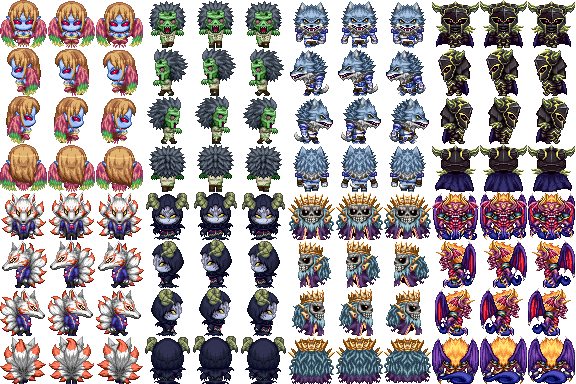
\includegraphics[width=4cm]{Enemigos.png}
	\centering
\end{figure}

\subsubsection*{Motion}
Clase padre que heredara la clase Sprite. Le dará sprites y movimiento a sus clases hijas.\newline

\subitem \textbf{Propiedades:} \newline
* masa.
* r: Vector posición.\newline
* v: Vector velocidad.\newline
* a: Vector aceleración. \newline

\subitem \textbf{Funciones e interacciones:} \newline
* move(). \newline
* calculateAceleration(): calcula la aceleración dependiendo del tipo de movimiento. \newline

\subsubsection*{HealthBar}
Incluira QGraphicsRectItem y QGraphicsTextItem, consistirá en dos rectángulos, uno rojo y otro gris cuyos tamaños dependerán de la salud actual del personaje. \newline
\subitem \textbf{Propiedades:} \newline
* int health: cantidad de vida actual de personaje.\newline
* QGraphicsRectItem bar: rectángulo cuyo ancho dependerá de cuanta salud le quede al personaje.\newline
* QGraphicsTextItem textBar: texto que mostrara el por ciento de vida del personaje, este texto estará superpuesto sobre bar. \newline
* healthMax: maxima cantidad de vida. \newline
* QGraphicsRectItem barLose: rectángulo que dependerá de la vida perdida del personaje.\newline

\subitem \textbf{Funciones e interacciones:} \newline
Interactuara directamente con el player o con el enemigo, al momento de recibir daño o curar se actualizara la HealthBar
* updateBarHealth: actualiza la barra de vida. \newline
* updateBarLoseHealth: actualiza la barra de vida perdida. \newline
* increase(int cure): Incrementa la vida y actualiza las barras. \newline
* decrease(int damage): decrementa la vida y actualiza las barras. \newline

\subsubsection*{Player}
Heredara Motion. sera manejado por el usuario, tendrá el focus del teclado. \newline
\subitem \textbf{Propiedades:} \newline
* bool state: si esta vivo o muerto.\newline
* HealthBar health: sera la barra de vida del personaje.\newline
* Weapon weapon: arma equipada.\newline
* int flechas: cantidad de flechas que tiene actualmente.\newline
* Bool arco: si tiene arco.\newline
* Bool dash: si tiene el dash.\newline
* Bool invertGravity: si tiene invertir gravedad\newline
* Bool inmu: si es inmune al daño o no.\newline
* int potions: cantidad de pociones.\newline

\begin{figure}[!ht]
	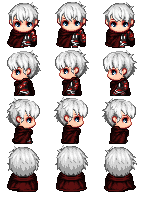
\includegraphics[width=4cm]{personaje.png}
	\centering
\end{figure}

\subitem \textbf{Funciones e interacciones:} \newline
Player interactuara con los enemigos, bloques, sierras, péndulos,  habilidades, atacar con el arma equipada y disparar un arco.
* dieAnimation: animación de muerte.\newline
* cure(Potion): Usa una poción para curarse. esto modifica la barra de vida del personaje.\newline
* attack(Weapon): ataca con el arma equipada.\newline
* damage(Enemy, Block, Saw, Pendulum, arrow): recibe daño que disminuye su barra de vida y le da frames de invulnerabilidad.\newline
* shoot(Bow): usa un arco para disparar una flecha.\newline
* dash(Dash): realiza un dash y le da frames de invulnerabilidad contra ciertos objetos.\newline
* doubleJump(DoubleJump):\newline
* invert(InvertGravity): invierte la gravedad.\newline

\subsubsection*{Enemy}
Heredara la clase motion, sera una clase padre, de la cual sus hijas serán todos los distintos tipos de enemigos que tendrán sus propios patrones de movimiento y de ataque.\newline

\subitem \textbf{Propiedades:} \newline
* HealthBar health: la misma que el jugador pero mas pequeña y dicha posición se ira actualizando con la posición del mismo enemigo.\newline
* bool state: si esta vivo o muerto.\newline
* atk: daño que hace al atacar\newline
* Bool inmu: Si es inmune al daño o no.\newline

\subitem \textbf{Funciones e interacciones:} \newline
Podra interactuar consigo mismo y con el player.\newline
* dieAnimation: Animación que se activa al perder toda la vida.\newline
* damage(): recibe daño.\newline
* attack(Player): ataca al jugador cuando esta en el rango, los ataques de cada tipo de enemigo serán distintos.\newline

\subsubsection*{Spike}
Heredara la clase Enemy. pinchos inmóviles que le hacen daño a Player al contacto.\newline

\subitem \textbf{Propiedades:} \newline
No tienen ninguna propiedad particular.

\subitem \textbf{Funciones e interacciones:} \newline
La única interacción sera con Player. \newline

\subsubsection*{Block}
Heredara motion. Clase padre de la cual heredaran los distintos tipos de bloques. Segun el tipo de bloque tendra movimiento.\newline
\subitem \textbf{Propiedades:} \newline
No tendrá propiedades aparte de las que hereda. \newline
\subitem \textbf{Funciones e interacciones:} \newline
Interactúa de manera pasiva con el jugador, con el enemigo y con las flechas. Destruye las flechas y supone un obstáculo tanto como para el jugador como para el enemigo. \newline
* destroyArrow(arrow): destruye una flecha.

\subsubsection*{Bow}
Heredara la clase Sprites. Servirá para dispara una flecha.\newline

\subitem \textbf{Propiedades:} \newline
* pot: Magnitud de un vector velocidad.\newline
* angle: Angulo del vector velocidad inicial de la flecha a disparar.\newline
* atk: daño que hace la flecha que dispara.\newline

\subitem \textbf{Funciones e interacciones:} \newline
El arco interactuara con el enemigo y el jugador, ya que ellos son los lo que lo usaran. También interactúa con las flecha, el arco es el que las dispara. \newline
* shoot(arrow): Dispara una flecha.\newline
* shoot(player, enemy): jugador o enemigo que dispara el arco.\newline

\subsubsection*{Arrow}
Heredara la clase motion. La flecha al ser disparada tendrá una velocidad inicial y una posición inicial dadas por el arco.\newline
\subitem \textbf{Propiedades:} \newline
* bool state.\newline
* bool type: si es disparada por el enemigo o por el jugador.\newline
* atk daño que hace al impacto.\newline
\subitem \textbf{Funciones e interacciones:} \newline
Interactua con Block, con Player y con Enemy. \newline
* destroyAnimation: animación al destruirse contra un bloque. \newline
* damage(personaje, enemigo): hará daño al jugador o enemigo dependiendo quien la disparo. \newline


\subsubsection*{Potion}
Heredara la clase Sprite. \newline

\subitem \textbf{Propiedades:} \newline
* pot: cantidad de vida que recupera al usarse. \newline

\subitem \textbf{Funciones e interacciones:} \newline
Interactúa con la HealthBar.\newline
* animation(): animación que se activa al usarse. \newline
* cure(healthBar): Cura la vida del Player/HealthBar. \newline

\subsubsection*{Saw}
Hereda de la clase enemigo. Habran cierras inmóviles, móviles y de distintos tamaños. Tendrá un movimiento circular uniforme sobre si misma que dará el efecto de ser una sierra cortante.\newline 

\subitem \textbf{Propiedades:} \newline
* HitBox: se refinara la hitbox para que sea exactamente la de un circulo.\newline
Tendrá las propiedades necesarias para simular el movimiento circular sobre su propio eje.\newline

\subitem \textbf{Funciones e interacciones:} \newline
Al ser hija de enemigo, interactúa con Player y con los Enemy que sean de un tipo diferente a Saw. Todas las funciones necesarias ya están en Enemy.\newline

\subsubsection*{Pendulum}
Hereda de la clase Block y la clase Motion. sera un bloque con movimiento.\newline

\subitem \textbf{Propiedades:} \newline
* HitBox: se refinara la hitbox para que sea exactamente la de un circulo.\newline
En motion estará lo necesario para simular dicho movimiento.\newline
 
\subitem \textbf{Funciones e interacciones:} \newline
Mismas interacciones que la de un Block solo que su hitbox sera circular.

\subsubsection*{Dash}
Hereda la clase Sprites. Habilidad del personaje, al usarla este se moverá rápidamente hacia una dirección ignorando los efectos de la gravedad por un breve periodo de tiempo. \newline

\subitem \textbf{Propiedades:} \newline
* pot: Aumento de velocidad del personaje al usarla.\newline
* time: Duración del efecto.\newline
* state: Si esta disponible para usarla. Cada x tiempo después de usarse volverá a estado true.\newline

\subitem \textbf{Funciones e interacciones:} \newline
* animation(): Animación al usarla.\newline
* use(Player): Uso de dicha habilidad. El efecto terminara después de un breve periodo de tiempo o si choca contra un bloque. \newline

\end{document}
